% ============================================================
%  P6 -- Full-wave optical response of simulated Cu glancing-angle
%        films: FDTD on voxelised ballistic morphology versus
%        measured Mueller-matrix ellipsometry
%
%  Template: AIP Publishing (revtex4-1, aip class option)
%  Target: Optics Express / JOSA B / Optical Materials
%
%  FIRST DRAFT 2026-09-10 -- generated from:
%    05_THESIS_PAPER_ASSETS/P6_PHOTONICS_STATE_ASSESSMENT_20260908.md
%    .../figures/publication/optical_fdtd_pilot/P6_GAP1_MUELLER_RESULT_20260909.md
%    .../figures/publication/optical_fdtd_pilot/P6_GAP2_SWEEP_RESULT_20260909.md
%    P6_MANUSCRIPT_SKELETON_20260910.md
%  Numbers not recomputed for this draft. TODO(author): figures, venue,
%  abstract length, AI-disclosure wording, decide mm33/mm22 presentation.
% ============================================================
\documentclass[aip,jcp,amsmath,amssymb,reprint]{revtex4-1}
\usepackage{graphicx}
\usepackage{siunitx}
\usepackage{booktabs}
\graphicspath{{../figures/publication/}}

\begin{document}

\title{Full-wave optical response of simulated Cu glancing-angle films:
FDTD on voxelised ballistic morphology versus measured Mueller-matrix
ellipsometry}

\author{Oussama Ben Haj Ali}
\affiliation{Laboratoire de Photovolta\"{i}que et Mat\'{e}riaux Semi-conducteurs (LPMS),
\'{E}cole Nationale d'Ing\'{e}nieurs de Tunis (ENIT), Universit\'{e} de Tunis El Manar, Tunisia}
\author{Bruno Gallas}
\affiliation{Institut des NanoSciences de Paris (INSP), CNRS, Sorbonne Universit\'{e}, Paris, France}
\author{Ferid Chaffar Akkari}
\affiliation{Laboratoire de Photovolta\"{i}que et Mat\'{e}riaux Semi-conducteurs (LPMS),
\'{E}cole Nationale d'Ing\'{e}nieurs de Tunis (ENIT), Universit\'{e} de Tunis El Manar, Tunisia}

\date{\today}

\begin{abstract}
The optical anisotropy of glancing-angle-deposition (GLAD) films is usually
modelled with effective-medium approximations or idealised tilted cylinders. We
instead run finite-difference time-domain (FDTD) electromagnetic simulations
directly on the voxelised morphology of a ballistic GLAD growth model, with a
reflection-accounting Nicolson--Ross--Weir index retrieval validated to
\SI{0.1}{\percent} on a known dielectric slab, tabulated Lorentz--Drude and
literature dispersion for the constituent materials, and an oxide core--shell
geometry. Comparing to a real Cu GLAD film measured by Mueller-matrix
ellipsometry, a three-realisation average of the non-depolarising Mueller
elements moves three of four adjustable elements toward the measured, genuinely
depolarised values, while one element moves the wrong way and the largest
depolarisation signature cannot be reproduced by realisation averaging at all --
a first-principles incoherent-sum formulation is required. A nine-angle sweep on
grid-rebuild-corrected voxels gives a physically sane, monotonically increasing
void fraction with deposition angle and an effective index consistent in
direction, though not magnitude, with a published Cu$_2$O optical Bruggeman
trend. The results establish that full-wave modelling on the true simulated
morphology is tractable and partially reproduces measured optical anisotropy,
and they identify depolarisation modelling as the principal open problem.
\end{abstract}

\maketitle

% ============================================================
\section{Introduction}
\label{sec:intro}
GLAD films are optically anisotropic and, at high deposition angle, partially
depolarising. Their optical response is most often modelled either with an
effective-medium approximation (Bruggeman, Maxwell--Garnett) applied to a
porosity estimate, or with full-wave calculations on an idealised geometry of
tilted cylinders. Neither uses the actual film morphology, and neither naturally
produces depolarisation. Here we take the morphology produced by a validated
ballistic GLAD growth model, voxelise it, and run full-wave FDTD directly on it,
with realistic material dispersion and an oxide shell, and we compare the result
to a real Cu GLAD film measured by Mueller-matrix ellipsometry.

% ============================================================
\section{Methods}
\label{sec:methods}

\subsection{Morphology}
Film morphology is taken from the ballistic bead model of the companion paper,
at atomic radius \SI{0.128}{nm}, using the grid-rebuild-corrected engine build.
The atomic configuration is voxelised; an oxide core--shell is applied with a
shell thickness taken from a prior thickness sweep.

\subsection{FDTD and index retrieval}
FDTD is performed with MEEP. The effective index is retrieved from the complex
reflection and transmission with a Nicolson--Ross--Weir procedure that accounts
for multiple internal reflections; on a known $\varepsilon = 4$ slab this
retrieval is accurate to \SI{0.1}{\percent}, against roughly \SI{5}{\percent}
for a Born approximation. Both linear polarisations are computed. Material
dispersion uses a Lorentz--Drude fit for tungsten \citep{rakic1998optical} and
literature optical constants for Cu$_2$O \citep{malerba2011cu2o}, cross-checked
against an independent REELS-based tungsten dataset (Werner \textit{et al.},
2009) that disagrees with the Rakic/Palik consensus value at 500\,nm by a
known, technique-dependent margin.

\subsection{Measured reference}
The experimental reference is a Cu GLAD film measured by spectroscopic
Mueller-matrix ellipsometry (INSP, dataset \texttt{test10.dat}), which shows
genuine depolarisation.

% ============================================================
\section{Results}
\label{sec:results}

\subsection{Mueller-matrix comparison and the depolarisation problem}
\label{ssec:mueller}
Table~\ref{tab:mueller} compares the measured non-zero Mueller elements at
$\alpha = \ang{85}$ to a single simulated realisation and to an average over
three independent realisations (seeds 000/001/002).

\begin{table}[t]
\caption{Measured versus simulated Mueller elements at $\alpha = \ang{85}$.
Three of four adjustable elements move toward the measured value under
three-realisation averaging; mm33 moves away; mm22 is fixed at \num{1.0} by the
non-depolarising conversion and cannot move.}
\label{tab:mueller}
\begin{ruledtabular}
\begin{tabular}{lccc}
element & measured & single realisation & 3-seed average \\
\colrule
mm12 & $-0.658$ & $-0.898$ & $-0.876$ \\
mm21 & $-0.669$ & $-0.898$ & $-0.876$ \\
mm33 & $\phantom{-}0.325$ & $\phantom{-}0.300$ & $\phantom{-}0.382$ \\
mm34 & $\phantom{-}0.598$ & $-0.321$ & $-0.291$ \\
mm22 & $\phantom{-}0.943$ & $\phantom{-}1.000$ & $\phantom{-}1.000$ \\
\end{tabular}
\end{ruledtabular}
\end{table}

The movements toward the measured values are small -- a few percent of the total
measured-to-simulated gap -- and mm33 moves the wrong way. mm34 improves in
magnitude but retains an unresolved sign discrepancy tied to the retardance
sign convention. Most importantly, mm22 equals \num{1.0} exactly for every
individual realisation by construction of the non-depolarising Mueller
conversion, so its average over any number of realisations is also \num{1.0};
this procedure cannot reproduce the largest measured depolarisation signature
(\num{0.943} versus the non-depolarising baseline \num{1.0}), visualised in
Fig.~\ref{fig:mueller}. A genuine
depolarisation calculation requires a first-principles incoherent-sum or
partial-coherence FDTD formulation rather than an average of per-realisation
non-depolarising conversions.

\begin{figure}[t]
\centering
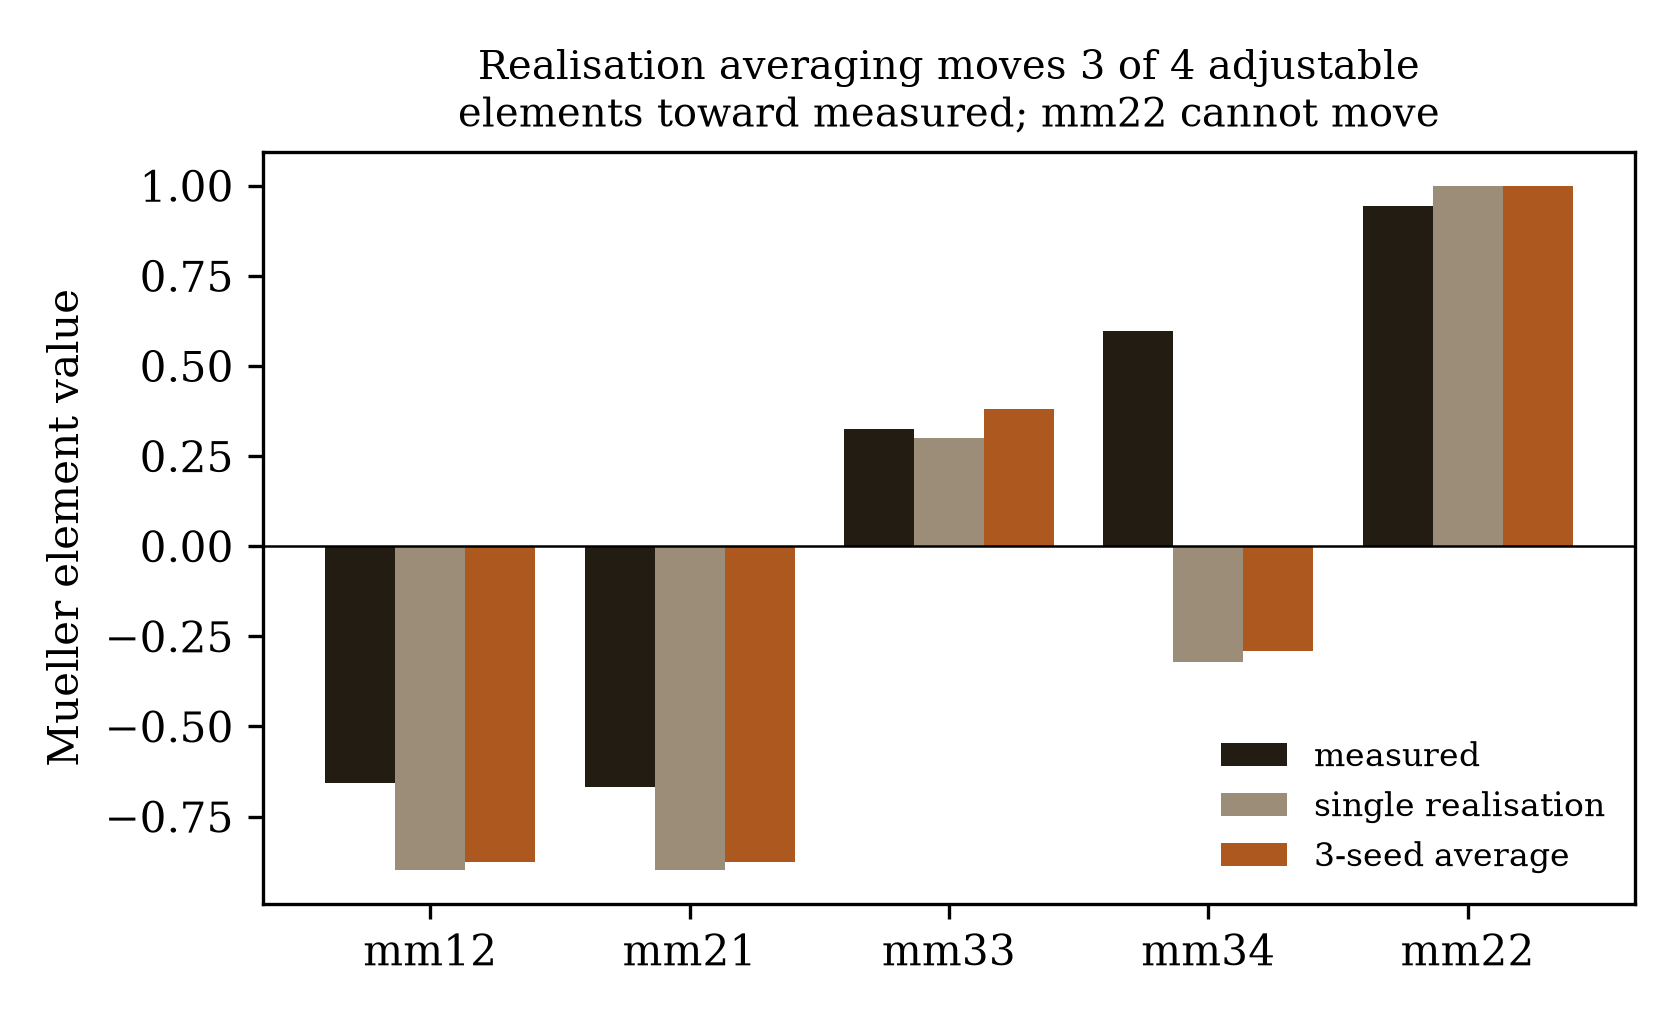
\includegraphics[width=0.9\linewidth]{P6_mueller_comparison}
\caption{Measured versus simulated Mueller elements at $\alpha=\ang{85}$
(same numbers as Table~\ref{tab:mueller}). Three of four adjustable
elements move toward the measured value under 3-seed averaging; mm22 is
fixed at 1.0 by construction and cannot reproduce the measured
depolarisation.}
\label{fig:mueller}
\end{figure}

With $n = 3$ realisations the spread across seeds
is indicative, not a converged uncertainty; the direction of movement is the
reportable finding, not the precise magnitudes.

\subsection{Angle sweep on corrected voxels}
\label{ssec:sweep}
A nine-angle sweep ($\alpha = 60$--\ang{89}) was run on grid-rebuild-corrected
voxels at \SI{0.128}{nm} atomic radius, both polarisations, in about
\SI{109}{min} of wall-clock. The $\alpha = \ang{60}$ point is excluded: the
corrected re-run gives a \SI{58}{\percent} solid fraction against an implausible
\SI{0.2}{\percent} before correction and against this project's own bulk
void-fraction table -- a qualitative voxelisation artefact at \ang{60} that the
companion paper already documents and excludes. The remaining eight angles
(Table~\ref{tab:sweep}, Fig.~\ref{fig:sweep}) give a void fraction that
increases with deposition angle, the expected shadowing direction (one
exception, $\alpha=\ang{72}\to\ang{75}$: a \SI{0.3}{pp} decrease within the
noise floor of the single-cross-section method), while the imaginary part
of the effective index falls correspondingly as the film becomes more
void-dominated.

\begin{figure}[t]
\centering

\includegraphics[width=0.9\linewidth]{P6_angle_sweep}
\caption{Void fraction and effective-index imaginary part versus deposition
angle on grid-rebuild-corrected voxels (same numbers as
Table~\ref{tab:sweep}).}
\label{fig:sweep}
\end{figure}

\begin{table}[t]
\caption{Angle sweep on corrected voxels (single mid-plane cross-section,
illustrative tungsten optical constants). $\alpha = \ang{60}$ excluded as a
voxelisation artefact.}
\label{tab:sweep}
\begin{ruledtabular}
\begin{tabular}{cccc}
$\alpha$ (deg) & void fraction & $n_\mathrm{eff}$ (real) & $n_\mathrm{eff}$ (imag) \\
\colrule
65 & \SI{50.9}{\percent} & 0.818 & 1.602 \\
70 & \SI{58.0}{\percent} & 0.777 & 1.442 \\
72 & \SI{65.4}{\percent} & 0.735 & 1.258 \\
75 & \SI{65.1}{\percent} & 0.736 & 1.265 \\
80 & \SI{80.2}{\percent} & 0.672 & 0.786 \\
85 & \SI{90.8}{\percent} & 0.750 & 0.329 \\
87 & \SI{92.9}{\percent} & 0.798 & 0.238 \\
89 & \SI{98.7}{\percent} & 0.962 & 0.036 \\
\end{tabular}
\end{ruledtabular}
\end{table}

Ben Nacer \textit{et al.}~\citep{bennacer2019cu2oglad} report a Cu$_2$O
optical Bruggeman porosity rising from \SI{23}{\percent} to \SI{37}{\percent}
over $\alpha = 0$--\ang{85}.
The present sweep rises far more steeply. The two use different techniques (a
single coherent two-dimensional cross-section threshold here versus a Bruggeman
fit to measured ellipsometric spectra) and different materials (illustrative
tungsten constants on Cu-derived morphology here versus real Cu$_2$O), so this
is a same-direction consistency check, not a validated quantitative match.

% ============================================================
\section{Discussion}
\label{sec:discussion}
Full-wave FDTD on the true voxelised ballistic morphology, with validated index
retrieval, realistic dispersion, and an oxide shell, is tractable and
partially reproduces the measured Mueller-matrix anisotropy of a real Cu GLAD
film. The results are honestly mixed: three of four adjustable non-depolarising
elements improve under realisation averaging, one worsens, and the dominant
depolarisation channel is inaccessible to the averaging method used. The angle
sweep is qualitatively correct but not a quantitative optical validation given
the cross-section convention and the illustrative optical constants.

The clearest lesson is methodological. Depolarisation in these films is real and
sizeable, and it will not emerge from averaging non-depolarising per-realisation
conversions; it requires a first-principles incoherent-sum treatment. Whether
the residual mm33 discrepancy is physical or numerical, and whether the mm34
sign issue is purely a convention, are the specific open questions.

% ============================================================
\section{Conclusion}
\label{sec:conclusion}
We have shown that finite-difference time-domain modelling on voxelised
ballistic GLAD morphology, compared against measured Mueller-matrix
ellipsometry, reproduces the direction of the measured optical anisotropy in
most channels after a grid-rebuild correction to the input morphology, while
leaving depolarisation as the principal unsolved problem. The infrastructure --
validated retrieval, real dispersion, real morphology, real measured reference
-- is in place; a first-principles depolarisation formulation and more
realisations are the next steps.

% ============================================================
\section*{Declaration on the use of AI tools}
% DRAFT 2026-09-10 -- authors to confirm the model list, task scope, and placement
% before submission. Policy basis: ../guide of writing articles with AI/WRITING_AND_AI_DISCLOSURE_GUIDE.md sec.8.
During the preparation of this work the authors used large language models
(Anthropic Claude; and, for bulk literature summarisation only, additional
models accessed through free-tier APIs) to assist with drafting and editing
prose, generating and refactoring analysis and simulation code, structuring
arguments, and summarising background literature. All AI-assisted text, code,
numerical results, and references were subsequently reviewed and verified by the
authors against primary sources or independent computation, and edited as
needed. The authors take full responsibility for the content of the publication.
No AI system is listed as an author, in line with COPE, ICMJE, and the relevant
publisher policies.

\section*{Declarations}

\begin{itemize}
\item \textbf{Funding:} No specific financial support statement is declared
  for this manuscript because no verified project number, contract number, or
  funding-agency wording was found in the local project records.
\item \textbf{Conflict of interest:} The authors declare no competing interests.
\item \textbf{Ethics approval and consent to participate:} Not applicable.
\item \textbf{Consent for publication:} Not applicable.
\item \textbf{Data availability:} The FDTD result files, the index-retrieval
  outputs, and the Mueller-matrix comparison tables supporting the findings
  of this study are permanently archived at Zenodo,
  DOI: \href{https://doi.org/10.5281/zenodo.22707349}{10.5281/zenodo.22707349}
  (concept DOI, resolves to the latest release), mirroring the GitHub
  repository \url{https://github.com/oussamabha/ballistic-GLAD-NIF}.
\item \textbf{Materials availability:} Not applicable.
\item \textbf{Code availability:} The FDTD scripts and the Nicolson--Ross--Weir
  retrieval code supporting the findings of this study are permanently
  archived at Zenodo,
  DOI: \href{https://doi.org/10.5281/zenodo.22707349}{10.5281/zenodo.22707349},
  mirroring the GitHub repository \url{https://github.com/oussamabha/ballistic-GLAD-NIF}.
\item \textbf{Author contribution:} O.B.H.A.: Conceptualization, Methodology,
  Software, Investigation, Formal analysis, Writing -- original draft. B.G.:
  Supervision, resources (ellipsometry), Writing -- review \& editing. F.C.A.:
  Supervision (principal), Writing -- review \& editing.
\end{itemize}

\bibliographystyle{aipnum4-1}
\bibliography{P6_references}

\end{document}
